\documentclass[xcolor=dvipsnames]{beamer}
\usepackage{calligra}
\usepackage{amsmath}
\usepackage{amsthm}
\usepackage{graphicx}
\usepackage{bm}
\usepackage{multimedia}
\usepackage{colortbl}

\usefonttheme{serif}
\usecolortheme[named=BrickRed]{structure}
\usetheme[height=7mm]{Rochester}
%\usetheme{default}
\title{\small{General Covariant Hamiltonian Approach\\to\\Generalized Harmonic Formulation of General Relativity}}
\author[M. Cao]{Meng Cao\\Advisor: Dr. John David Brown}
\institute[NCSU]{Department of Physics\\North Carolina State University\\Raleigh, NC 27695\\
\texttt{mcao2@ncsu.edu}}
\date[March 2014]{March 2014}
\begin{document}
	\begin{frame}
		\titlepage
	\end{frame}
	\begin{frame}{Outline}
		\begin{itemize}
			\item{Introduction}
			\item{Numerical Relativity}
			\item{General Covariance}
			\item{Hamiltonian Approach}
			\item{Summary and Future Work}
		\end{itemize}
	\end{frame}
	\begin{frame}{Introduction}
		\begin{itemize}
			\item{General Relativity}
			\item{Hamiltonian Formulation}
			%\item{Notation and Convention}
		\end{itemize}
	\end{frame}
	\begin{frame}{Introduction}
		General Relativity
		\begin{columns}[c]
			\column{2in}
			\begin{center}
				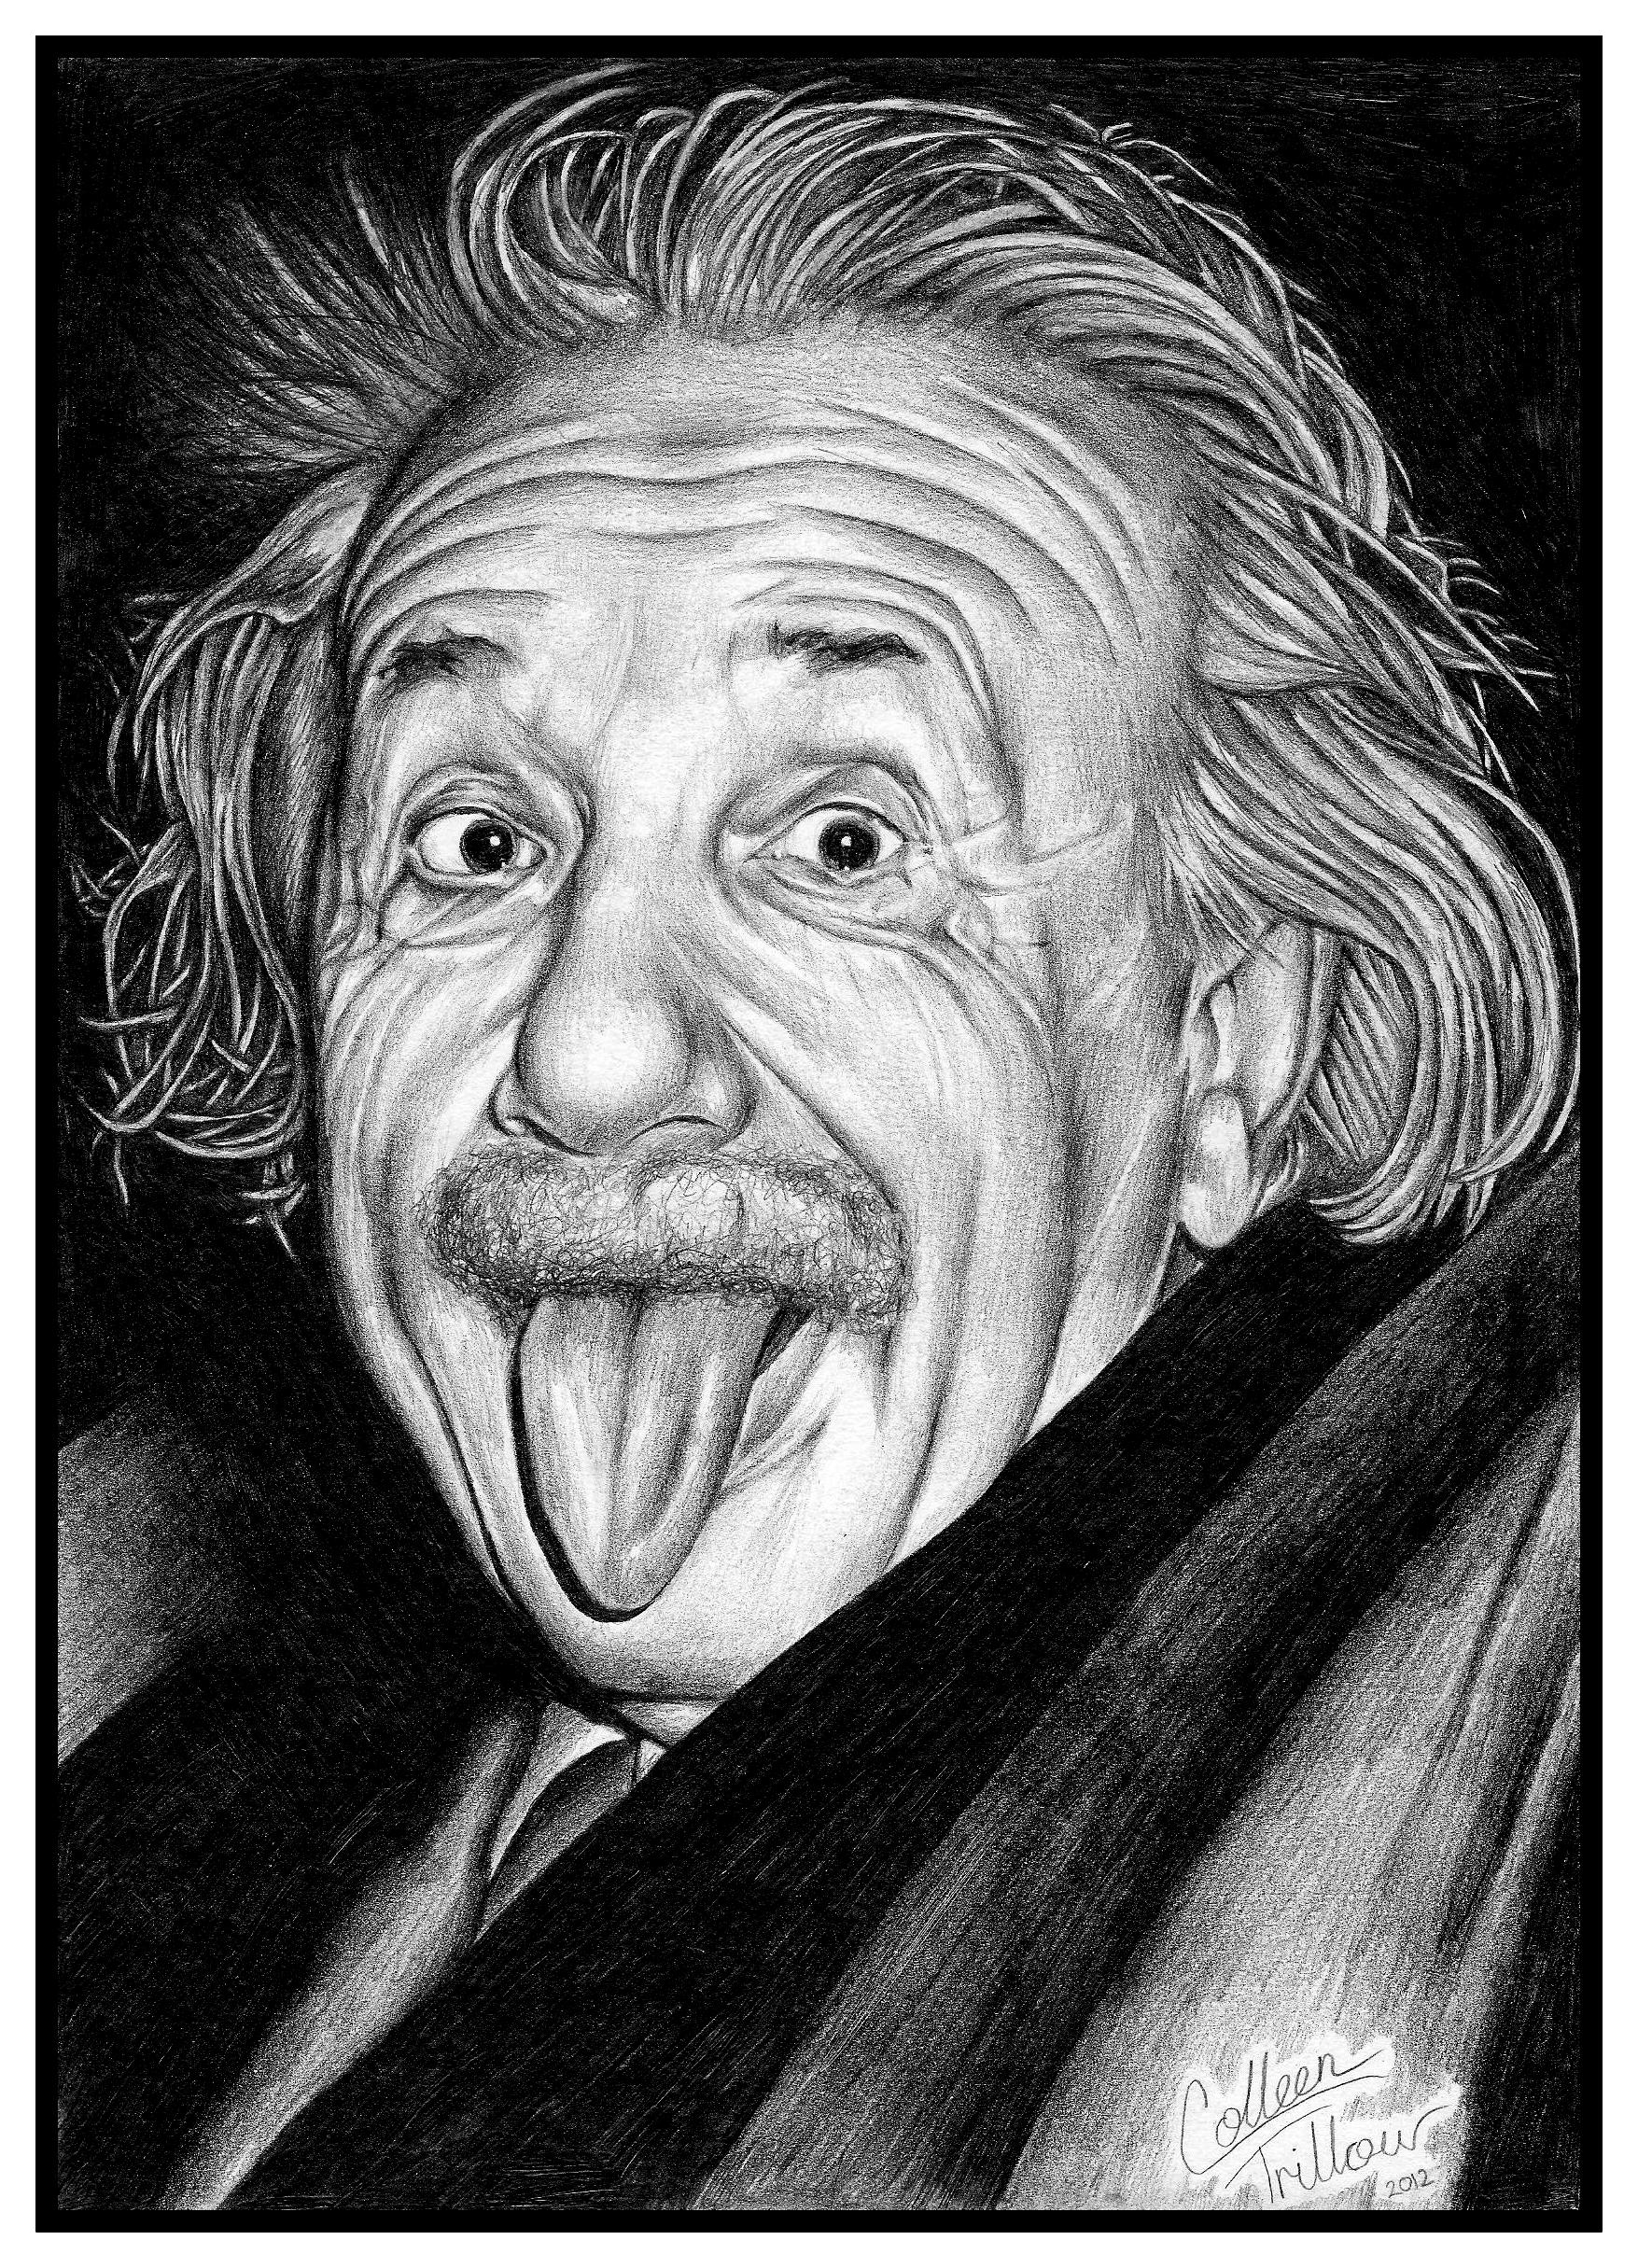
\includegraphics[scale=0.07]{einstein.jpg}\\
				\tiny{Colleen Trillow}
			\end{center}
			\column{2in}
			\begin{center}
				\includegraphics[scale=0.23]{grpaper.pdf}
			\end{center}
		\end{columns}
	\end{frame}
	\begin{frame}{Introduction}
		General Relativity
		\begin{center}
			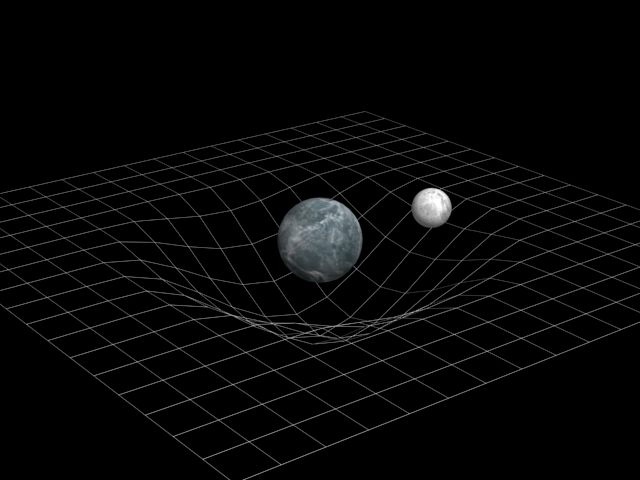
\includegraphics[scale=0.4]{curvature.jpg}
		\end{center}
	\end{frame}
	\begin{frame}{Introduction}
		Classical Tests of General Relativity
		\begin{itemize}
			\item{Light Deflection[Eddington, 1919]}
			\item{Perihelion Precession of Mercury[Urbain Le Verrier, 1859]}
			\item{Gravitational Redshift[Pound-Rebka, 1959]}
		\end{itemize}
	\end{frame}
	\begin{frame}{Introduction}
		Einstein Field Equations
		\huge
		\begin{center}
			\[
			G_{\mu\nu} = 8\pi T_{\mu\nu}
			\]
		\end{center}
	\end{frame}
	\begin{frame}{Introduction}
		Exact Solutions to Einstein Field Equations
		\begin{center}
			\Large
			\begin{tabular}{|c c c|}
				\hline
				\cellcolor[gray]{0.7}~ & \cellcolor[gray]{0.9}$J=0$ & $J \ne 0$ \\
				\rowcolor[gray]{0.9}$Q=0$ & \cellcolor[gray]{1.0}Schwarzschild & \cellcolor[gray]{0.7}Kerr \\
				\cellcolor[gray]{1.0}$Q\ne 0$ & \cellcolor[gray]{0.7}Reissner-Nordstr\"{o}m & \cellcolor[gray]{0.9}Kerr-Newman\\ \hline
			\end{tabular}
		\end{center}
	\end{frame}
	\begin{frame}{Introduction}
		Numerical Relativity
		\begin{columns}[c]
			\column{2in}
			\begin{center}
				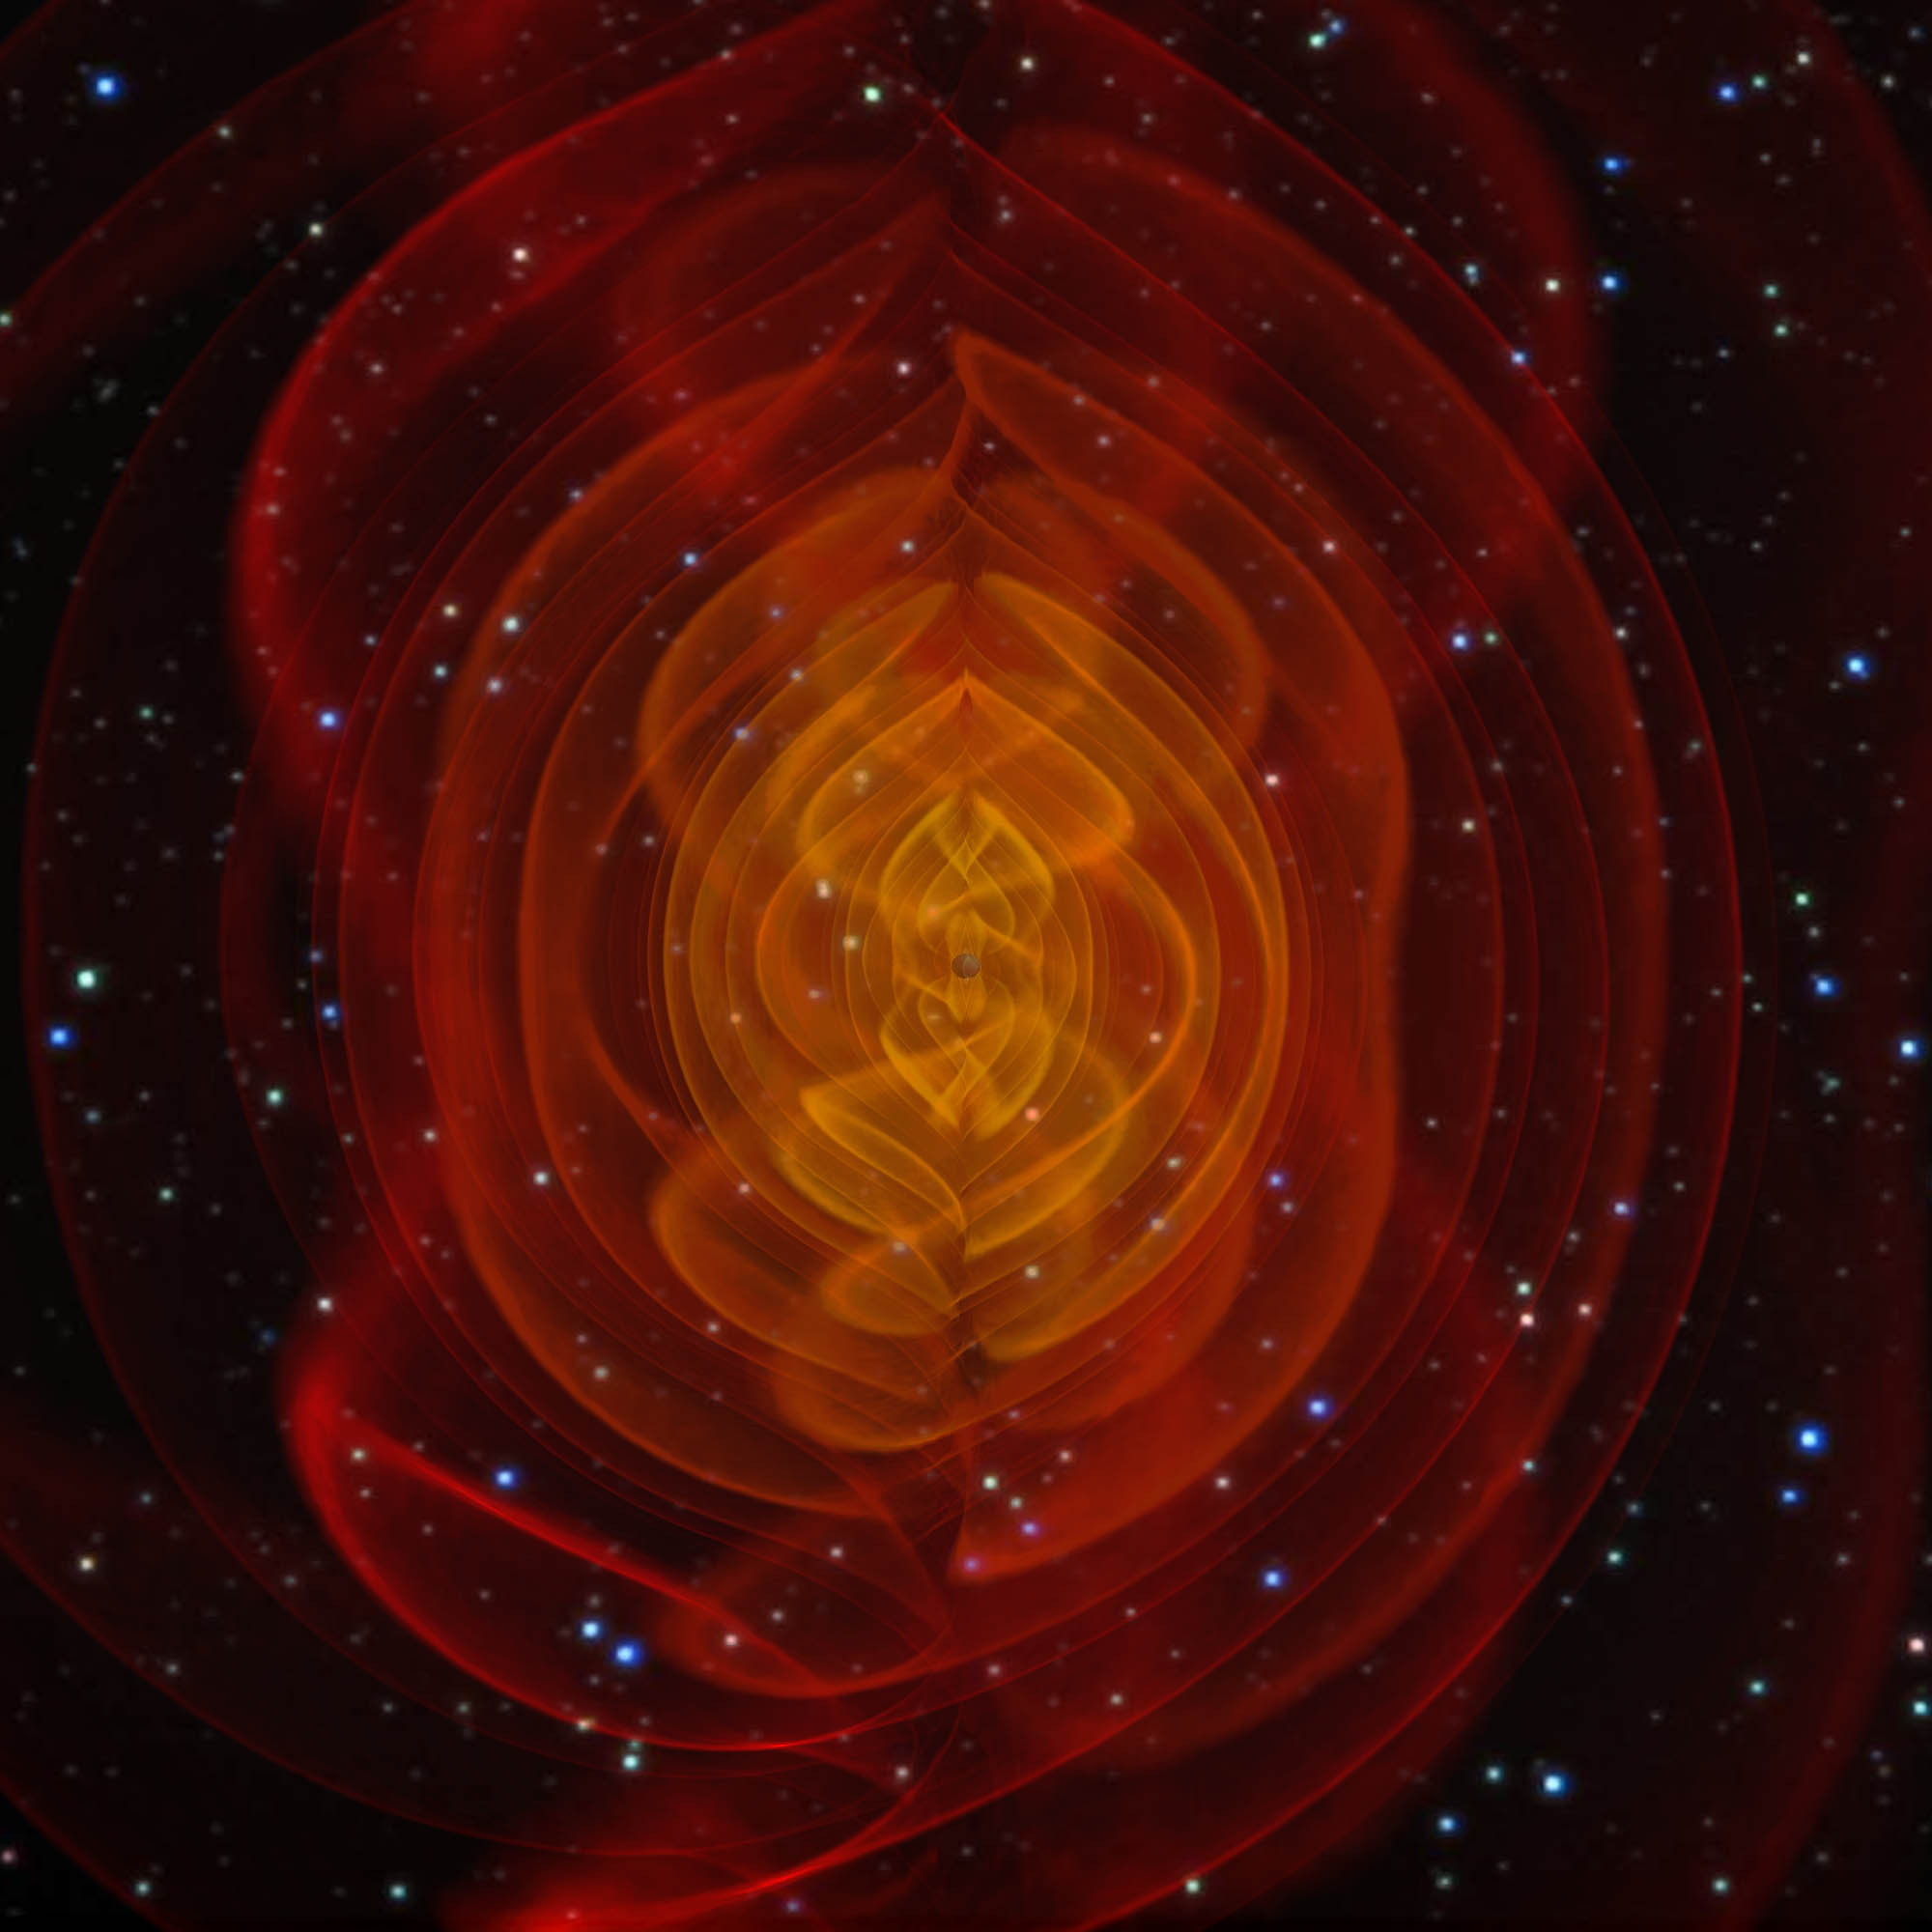
\includegraphics[scale=0.07]{nr-baker.jpg}\\
				\tiny{simulation: John Baker(NASA)}\\
				\tiny{visualization: Henze(NASA)}
			\end{center}
			\column{2in}
			\begin{center}
				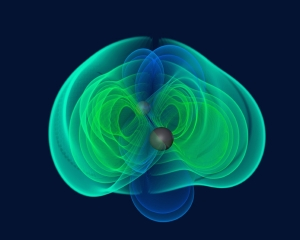
\includegraphics[scale=0.5]{nr-mpg.jpg}\\
				\tiny{simulation: C. Reisswig, L. Rezzolla(Albert Einstein Institute)}\\
				\tiny{visualization: M. Koppitz (Albert Einstein Institute/Zuse Institute Berlin)}
			\end{center}
		\end{columns}		
	\end{frame}
	\begin{frame}{Introduction}
		Hamiltonian Formulation
		\begin{center}
			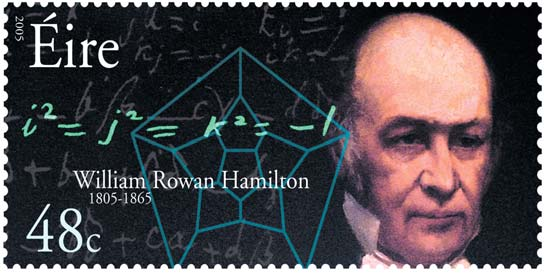
\includegraphics[scale=1.0]{hamilton.jpg}\\
			\tiny{Sir William Rown Hamilton(1805 - 1865)}
		\end{center}
	\end{frame}
	\begin{frame}{Introduction}
		Lagrangian vs Hamiltonian
		\begin{columns}[c]
			\column{2in}
			\begin{center}
				$\mathcal{L}(q_{i}, {\dot q}_{i}, t)$
				\begin{equation*}
					\frac{\partial}{\partial t}\frac{\partial \mathcal{L}}{\partial {\dot q_{i}}} - \frac{\partial \mathcal{L}}{\partial q_{i}} = 0
				\end{equation*}	
			\end{center}
			\column{2in}
			\begin{center}
				$\mathcal{H}(q_{i}, p_{i}, t)$	
				\begin{align*}
					{\dot p}_{i} + \frac{\partial \mathcal{H}}{\partial q_{i}} &= 0	\\
					{\dot q}_{i} - \frac{\partial \mathcal{H}}{\partial p_{i}} &= 0
				\end{align*}
			\end{center}
		\end{columns}
		\pause
		\begin{center}
			\Large{mathematically equivalent}
		\end{center}
	\end{frame}
	\begin{frame}{Introduction}
		Advantages of Hamiltonian Formulation
		\begin{itemize}
			\item{Equal Status of Coordinates and Momenta}
			\item{More Abstract Presentation of Physics}
			\item{Embarking Point of Modern Theories}
		\end{itemize}
	\end{frame}
	\begin{frame}{Numerical Relativity}
		\textbf{\textit{"If a corresponding large class of solutions of Einstein’s equation failed to exist, we would be forced to reject general relativity as a correct theory of nature"}}\\
		\hfill \textbf{--- Wald}
	\end{frame}
	\begin{frame}{Numerical Relativity}
		\begin{itemize}
			\item{3 + 1 Decomposition}
			\item{Numerical Formulations}
		\end{itemize}
	\end{frame}
	\begin{frame}{Numerical Relativity}
		3 + 1 Decomposition
		\begin{center}
			\Huge{\textbf{\textit{Demo}}}
		\end{center}
	\end{frame}
	\begin{frame}{Numerical Relativity}
		3 + 1 Decomposition
		\Large
		\[
		ds^{2} = - \alpha^{2}dt^{2} + g_{ab}(dx^{a} + \beta^{a}dt)(dx^{b} + \beta^{b}dt) 		
		\]
	\end{frame}
	\begin{frame}{Numerical Relativity}
		3 + 1 Decomposition
		\begin{center}
			\Large
			$g_{ab}~~~~\alpha~~~~\beta^{a}~~~~K_{ab}$
		\end{center}
	\end{frame}
	\begin{frame}
		Numerical Formulations
		\begin{itemize}
			\pause
			\item{ADM/BSSN}
			\pause
			\begin{itemize}
				\item{Arnowitt, Deser and Minser}
			\pause
				\item{Baumgarte, Shapiro, Shibata and Nakamura}
			\end{itemize}
			\pause
			\item{Generalized Harmonic}
			\pause
			\begin{itemize}
				\item{3 + 1 Form of GH Equations[Brown, 2011]}
				\item{Action Principle for GH formulation[Brown, 2011]}
			\end{itemize}
		\end{itemize}
	\end{frame}
	
\end{document}